\documentclass[a4paper]{article}

%% Language and font encodings
\usepackage[english]{babel}
\usepackage[utf8x]{inputenc}
\usepackage[T1]{fontenc}

%% Sets page size and margins
\usepackage[a4paper,top=3cm,bottom=2cm,left=3cm,right=3cm,marginparwidth=1.75cm]{geometry}

%% Useful packages
\usepackage{amsmath}
\usepackage{graphicx}
\usepackage[colorinlistoftodos]{todonotes}
\usepackage[colorlinks=true, allcolors=blue]{hyperref}

\title{Actividad 10}
\author{Isaac Neri Gómez Sarmiento}

\begin{document}
\maketitle


\section{Introducción}
Esta última actividad tiene como objetivo modificar parámetros de un modelo poblacional llamado mapeo logístico mediante el uso de WxMaxima con el fin de visualizar los efectos del caos en un sistema dinámico, como lo es una población, ya que por diversas causas, ésta cambia. Siendo más específicos, los sistemas caóticos son un subtipo de sistemas dinámicos no-lineales los cuales son dependientes de las condiciones iniciales. Cualquier cambio mínimo en las condiciones iniciales, conduce a un resultado muy diferente al pasar el tiempo. En pocas palabras, el caos se puede describir tal y como lo dijo el padre de la teoría del caos, Edward Lorenz, "Cuando el presente determina el futuro, pero el presente aproximado no determina aproximadamente el futuro".


\section{Comportamiento del sistema y atractores}

Para el modelado de una población, utilizaremos lo que se llama la función de mapeo logístico:\\

\begin{center}
$x_{t+1}=rx_t(1-x_t)$
\end{center}

Se le llama de mapeo logístico, porque mapea o asigna poblaciones conforme avanza cada paso de tiempo. La x representa la población a cualquier tiempo dado t y r representa la razón de crecimiento. El nivel de población en cualquier tiempo depdende o es función del parámetro de la razón de crecimiento  y la población anterior dada por el paso de tiempo anterior. 
Si el parámetro r es muy bajo, la población morirá y se extinguirá y si es muy alto, puede la población mantenerse estable o tener altibajos. Esta ecuación produce caos en ciertos valores para el parametro r.


La siguiente tabla presenta datos generados por la función de mapeo logístico. Se utilizaron 7 parámetros de crecimiento, 0.5, 1.0, 2.0, 2.5, 3.0 y 3.5.
Las columnas representan las razones de crecimiento, mientras que los renglones son el número de iteraciones. Se comienza con una población inicial de 0.5 y proporciona la población como proporción entre 0 y 1.


\begin{figure}[ht!]
\centering
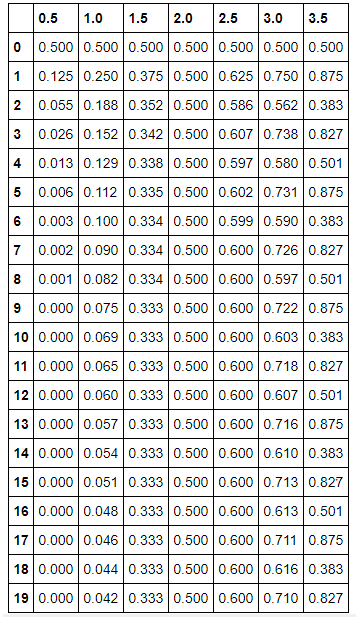
\includegraphics[width=0.45\textwidth]{Tabla.PNG}
\end{figure}
 
 \newpage

Las gráficas correspondientes a la tabla, para cada valor de razón de crecimiento se muestran:


\begin{figure}[ht!]
\centering
\includegraphics[width=50mm]{Logistic_model_r_0_5.PNG}
\includegraphics[width=50mm]{Logistic_model_r_1_0.PNG}
\includegraphics[width=50mm]{Logistic_model_r_1_5.PNG}
\includegraphics[width=50mm]{Logistic_model_r_2_0.PNG}
\end{figure}

\begin{figure}[ht!]
\centering
\includegraphics[width=50mm]{Logistic_model_r_2_5.PNG}
\includegraphics[width=50mm]{Logistic_model_r_3_0.PNG}
\includegraphics[width=50mm]{Logistic_model_r_3_5.PNG}
\end{figure}
\newpage

Podemos notar que para un valor de razón de crecimiento de 0.5, la población tiende a disminuir a cero. Para un valor de razón de crecimiento de 2.0, la población se mantiene estable. Para la gráfica con valor de razón de crecimiento de 3.0, parecen los valores ir convergiendo a un valor de población, mientras que para la gráfica con valor de razón de crecimiento de 3.5, simplemente rebota sin converger a un valor. Como pudimos, ver para un valor de razón de crecimiento de 0.5, el valor de la población converge a 0, a esto se le llama atractor, ya que es un valor o conjunto de valores al cual tiende un sistema converger al paso del tiempo.

\newpage

\section{Bifurcaciones y el Camino al Caos}

En esta ocasión se corrió el modelo 200 generaciones o iteraciones con 1000 razones de crecimiento entre 0.0 y 4.0. Para visualizar estos datos se necesitará de un diagrama de bifurcación:

\begin{figure}[ht!]
\centering
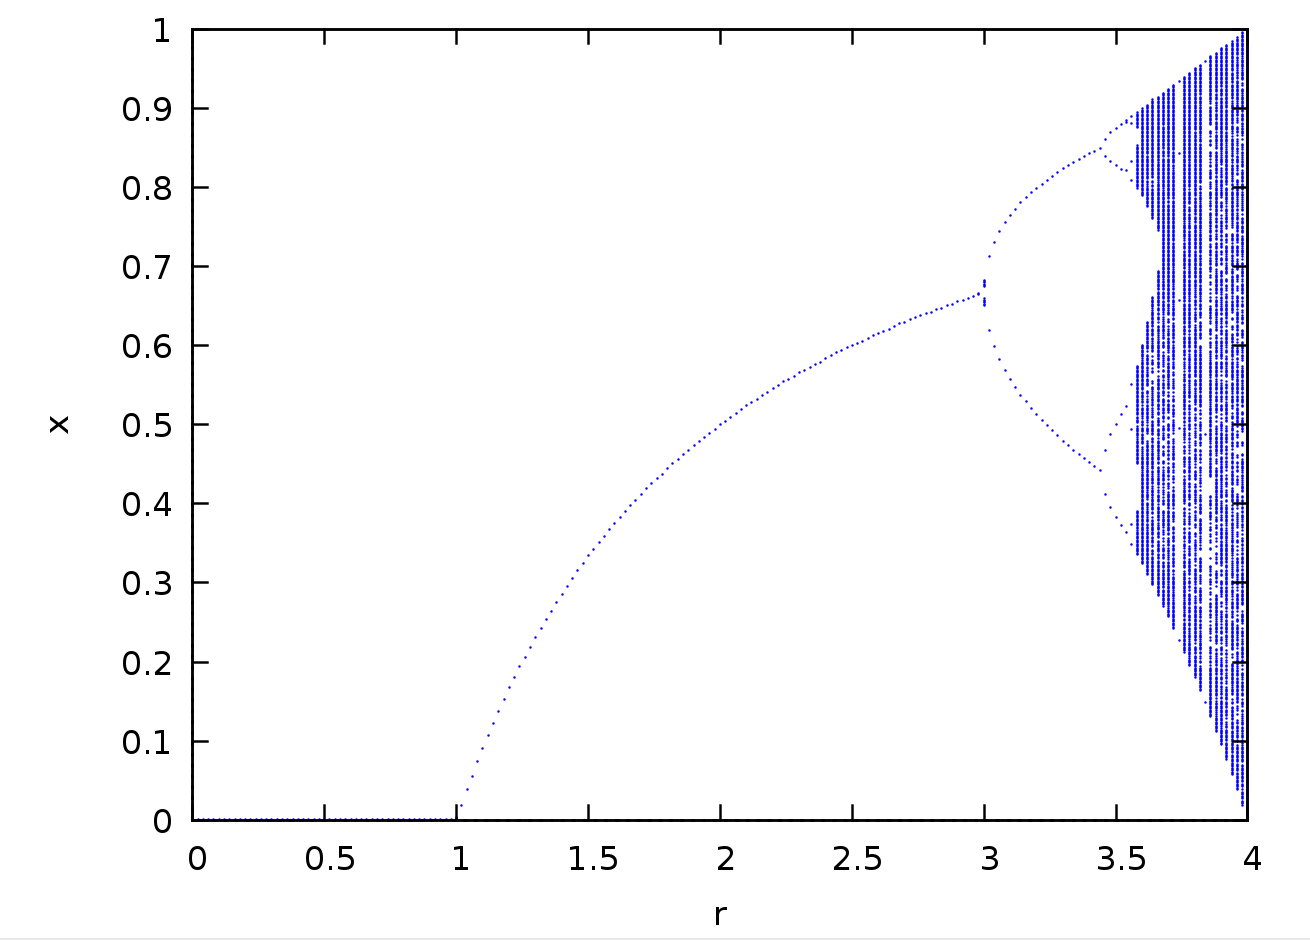
\includegraphics[width=0.45\textwidth]{Bifurcation1.png}
\end{figure}


Podemos ver que para razones de crecimiento menores que 1, el sistema siempre colapsa a cero, es decir la población se extingue. Para las razones de crecimiento entre 1.0 y 3.0, el sistema adopta un nivel de población estable.

En la siguiente gráfica se hace un acercamiento de la anterior pero en un intervalo de razón de de crecimiento de entre 2.8 y 4.0. 


\begin{figure}[ht!]
\centering
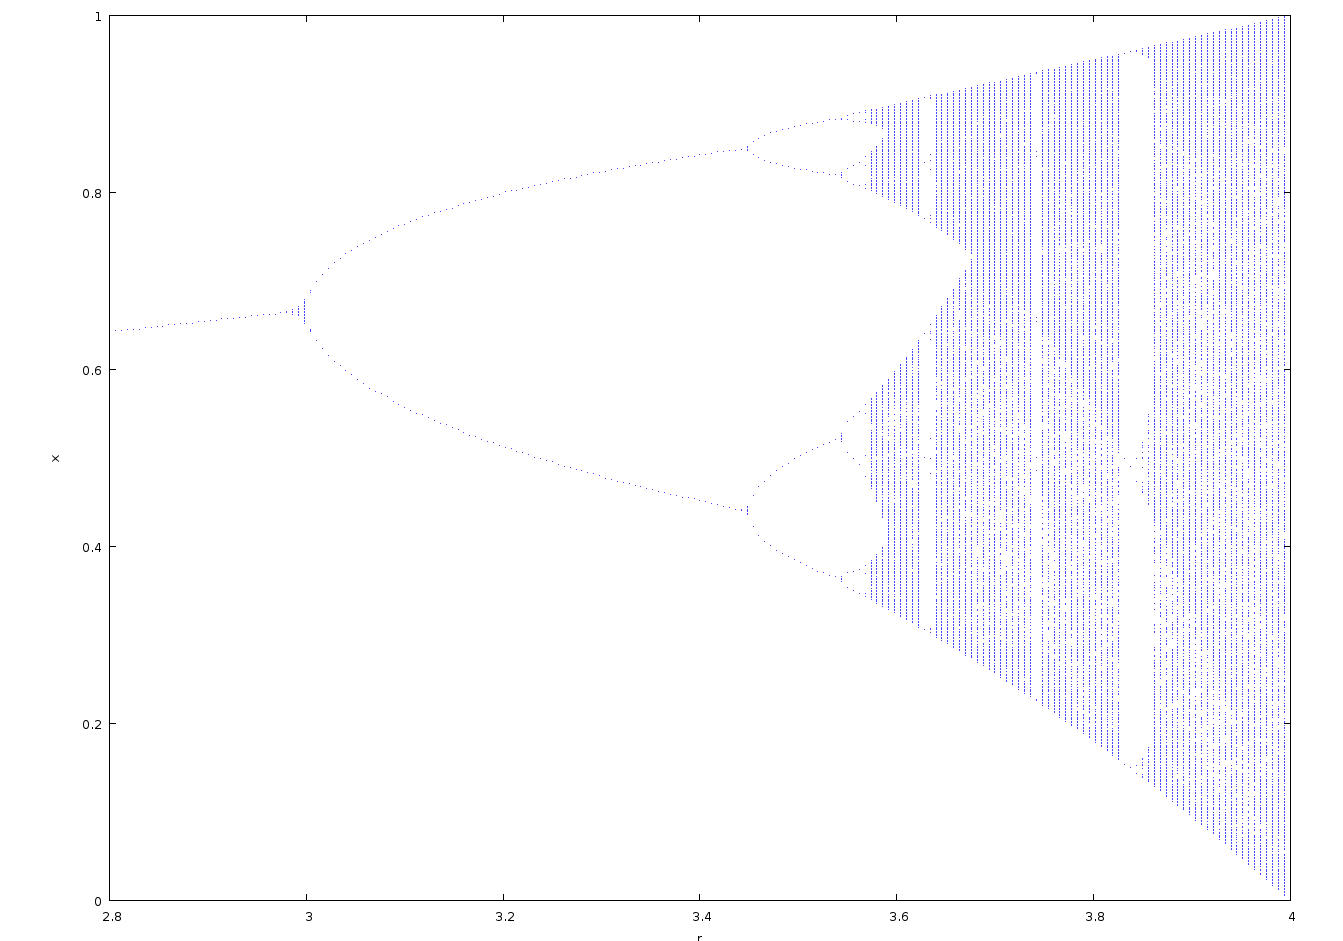
\includegraphics[width=0.6\textwidth]{Bifurcation2.png}
\end{figure}

Podemos notar que en la razón de crecimiento de 3, las poblaciones posibles se dividen en dos caminos.Para un valor del parámetro entre 3 y 3.43 aprox, el sistema oscila entre 0.5 y 0.8. El diagrama a su vez se divide en 4 caminos,y después de la razón de crecimiento de 3.5, los caminos se dividen en ocho.



\section{El comienzo del caos}

Mas allá de una razón de crecimiento de 3.6, las bifurcaciones incrementan hasta que el sistema es capaz de eventualmente parar en cualquier valor de población. A esto se le conoce como periodo de duplicación hacia el caos. Y este nombre se debe a que si sigues aumentando el parametro de razón de crecimiento, los valores de la población se irán duplicando: 2, 4, 8, 16, 32, etc. 

Veamos la gráfica de bifurcación ahora en un intervalo de 3.7 a 3.9 de la razón de crecimiento. 

\begin{figure}[ht!]
\centering
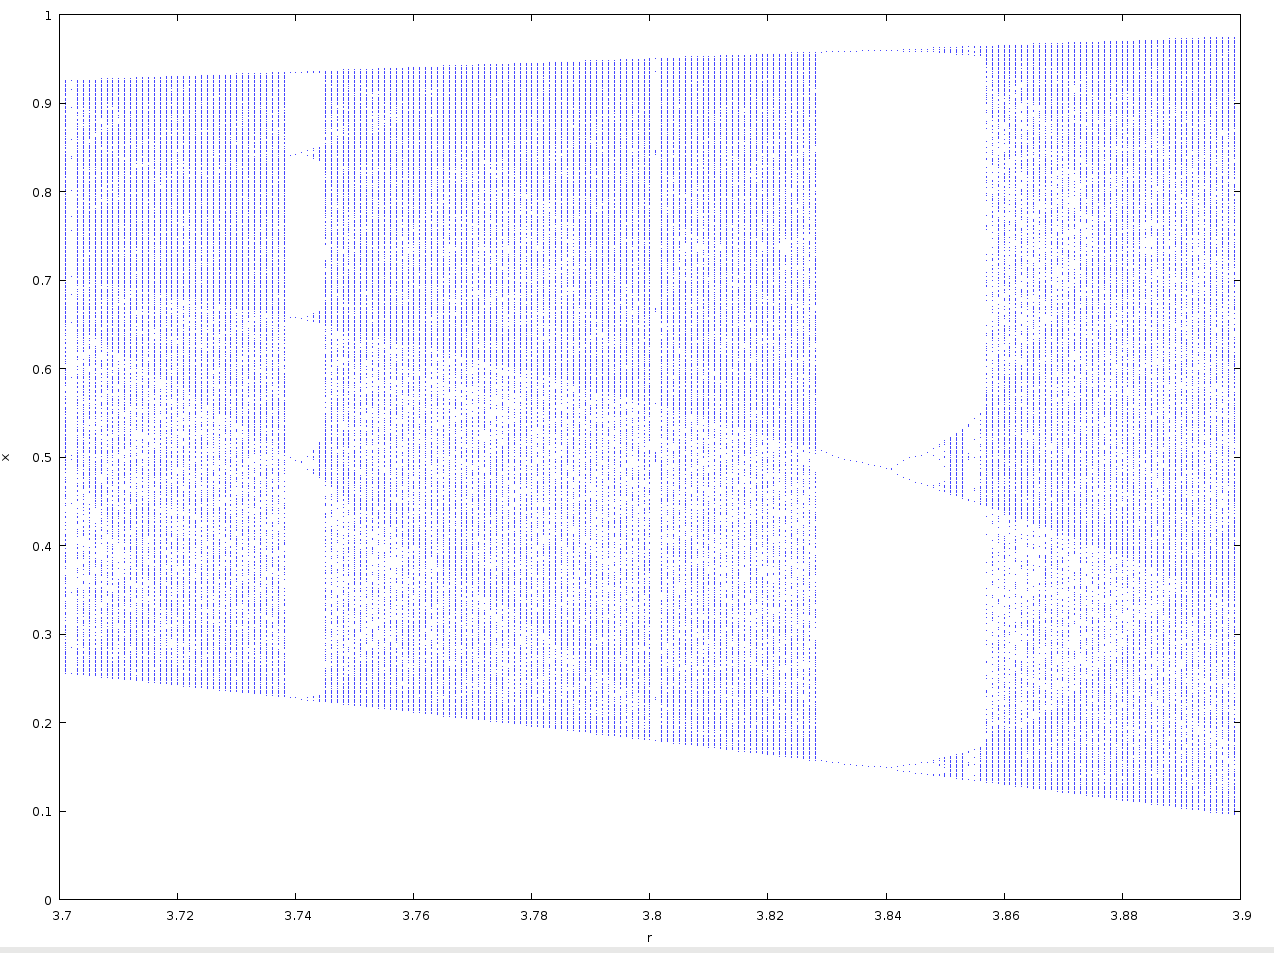
\includegraphics[width=0.6\textwidth]{Bifurcation3.png}
\end{figure}

Se puede notar que entre los parámetros de 3.82 y 3.84, el sistema es todo un caos y luego vuelve en orden, oscilando solamente entre tres valores de población, y luego se bifurca y regresa al caos el razones de crecimineto de 3.86.

\newpage
\section{Fractales y Atractores Extraños}


\begin{figure}[ht!]
\centering
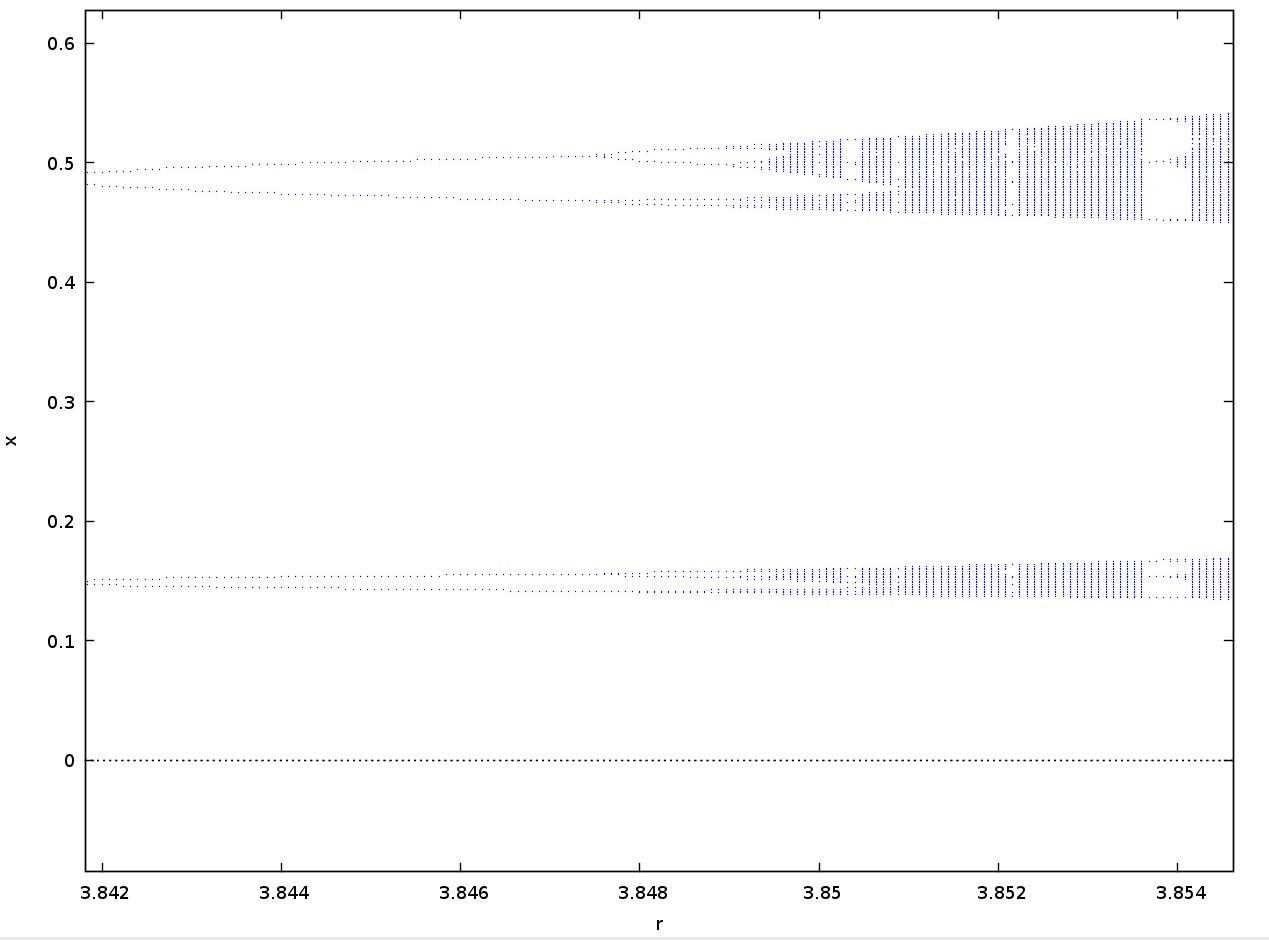
\includegraphics[width=0.6\textwidth]{Bifurcation4.png}
\end{figure}


En estas gráficas podemos encontrar fractales. Estas entidades son similares entre sí, y  vuelven a repetir el mismo patrón cuando se observa a diferentes escalas. Los sistemas caóticos tienen atractores extraños, alrededor de los cuales el sistema oscila para siempre, nunca repitiendose.

Otra manera de visualizar el sistema es con diagramas de fase, los cuales grafican el valor de población de la generación t+1 en el eje y, mientras que en el eje x grafica la población en la generación t.Son útiles para revelar atractores extraños en datos de series de tiempo. 


\section{El efecto Mariposa}

Recordemos que los sistemas caóticos son muy sensibles a las condiciones iniciales, por lo que para poder modelar y hacer predicciones de situaciones de la vida real se deben de medir los parámetros con una alta precisión, de otra manera por más pequeño que sea el error, a lo largo del tiempo empezarán a verse modificados los resultados. \\
Por ejemplo, si hacemos dos gráficas de población contra generación para valores de población inicial muy cercanos como 0.5 y 0.50001, obtenemos lo siguiente:



\begin{figure}[ht!]
\centering
\includegraphics[width=75mm]{pobl_in_0_5.PNG}
\includegraphics[width=71mm]{pobl_in_0_5001.PNG}

\end{figure}

Podemos notar que entre la generación 0 y 20 el comportamiento de las dos gráficas es el mismo. Pero, conforme va creciendo la generación, las poblaciones de ambos difieren. 

\newpage

\section{Conclusión}
Los sistemas caóticos son deterministas, es decir que si se utilizan varias veces un modelo con las mismas condiciones iniciales , se tendrán los mismos resultados y no serán al azar. Esto no implica que el comportamiento del modelo sea cíclico o que forme patrones periodicos. Se caracterizan algunos por tener atractores y fractales. Los atractores son valores los cuales tiende a converger el modelo al paso del tiempo, mientras que los fractales son entidades que tienen un patrón que se conserva a cualquier escala al alejarse o acercarse. El modelo de mapeo logístico es similar a una relación de recurrencia, en donde dado un valor inicial y algunos parámetros fijos, se pueden generar los siguientes valores de la secuencia, he de ahí que sea utilizado para modelar poblaciones.


\section{Bibliografía}

•Recurrence relation. Wikipedia. Recuperado el 24/05/2018 de: \url{https://en.wikipedia.org/wiki/Recurrence_relation} \\
•Chaos theory and the logistic map. Geoff Boeing. Recuperado el 24/05/2018 de: \url{http://geoffboeing.com/2015/03/chaos-theory-logistic-map/}\\
•Chaotic dynamics with Maxima.A. Morante y J. A. Vallejo. Recuperado el 24/05/2018 de: \url{https://arxiv.org/pdf/1301.3240.pdf}

\end{document}